
\addtocontents{toc}{\protect\setcounter{tocdepth}{0}}
\subsection{Rhombenkuboktaeder} \label{sec:rhombenkuboktaeder}
\addtocontents{toc}{\protect\setcounter{tocdepth}{3}}
Es gibt mehrere Möglichkeiten einen Rhombenkuboktaeder zu erstellen. Eine Möglichkeit ist es sich den Rhombenkuboktaeder in drei Ebenen vorzustellen: ein Prisma in der Mitte und zwei Dome (siehe Abbildung \ref{fig:rhombenkuboktaederToPseudorhombicuboctahedron}). Der Pseudo-Rhombenkuboktaeder entsteht dann durch Rotation einer der Dome um $\frac{2\pi}{8}=\frac{\pi}{4}$.

\begin{figure}[htp]
    \centering
    \begin{subfigure}[b]{0.32\textwidth}
        \centering
        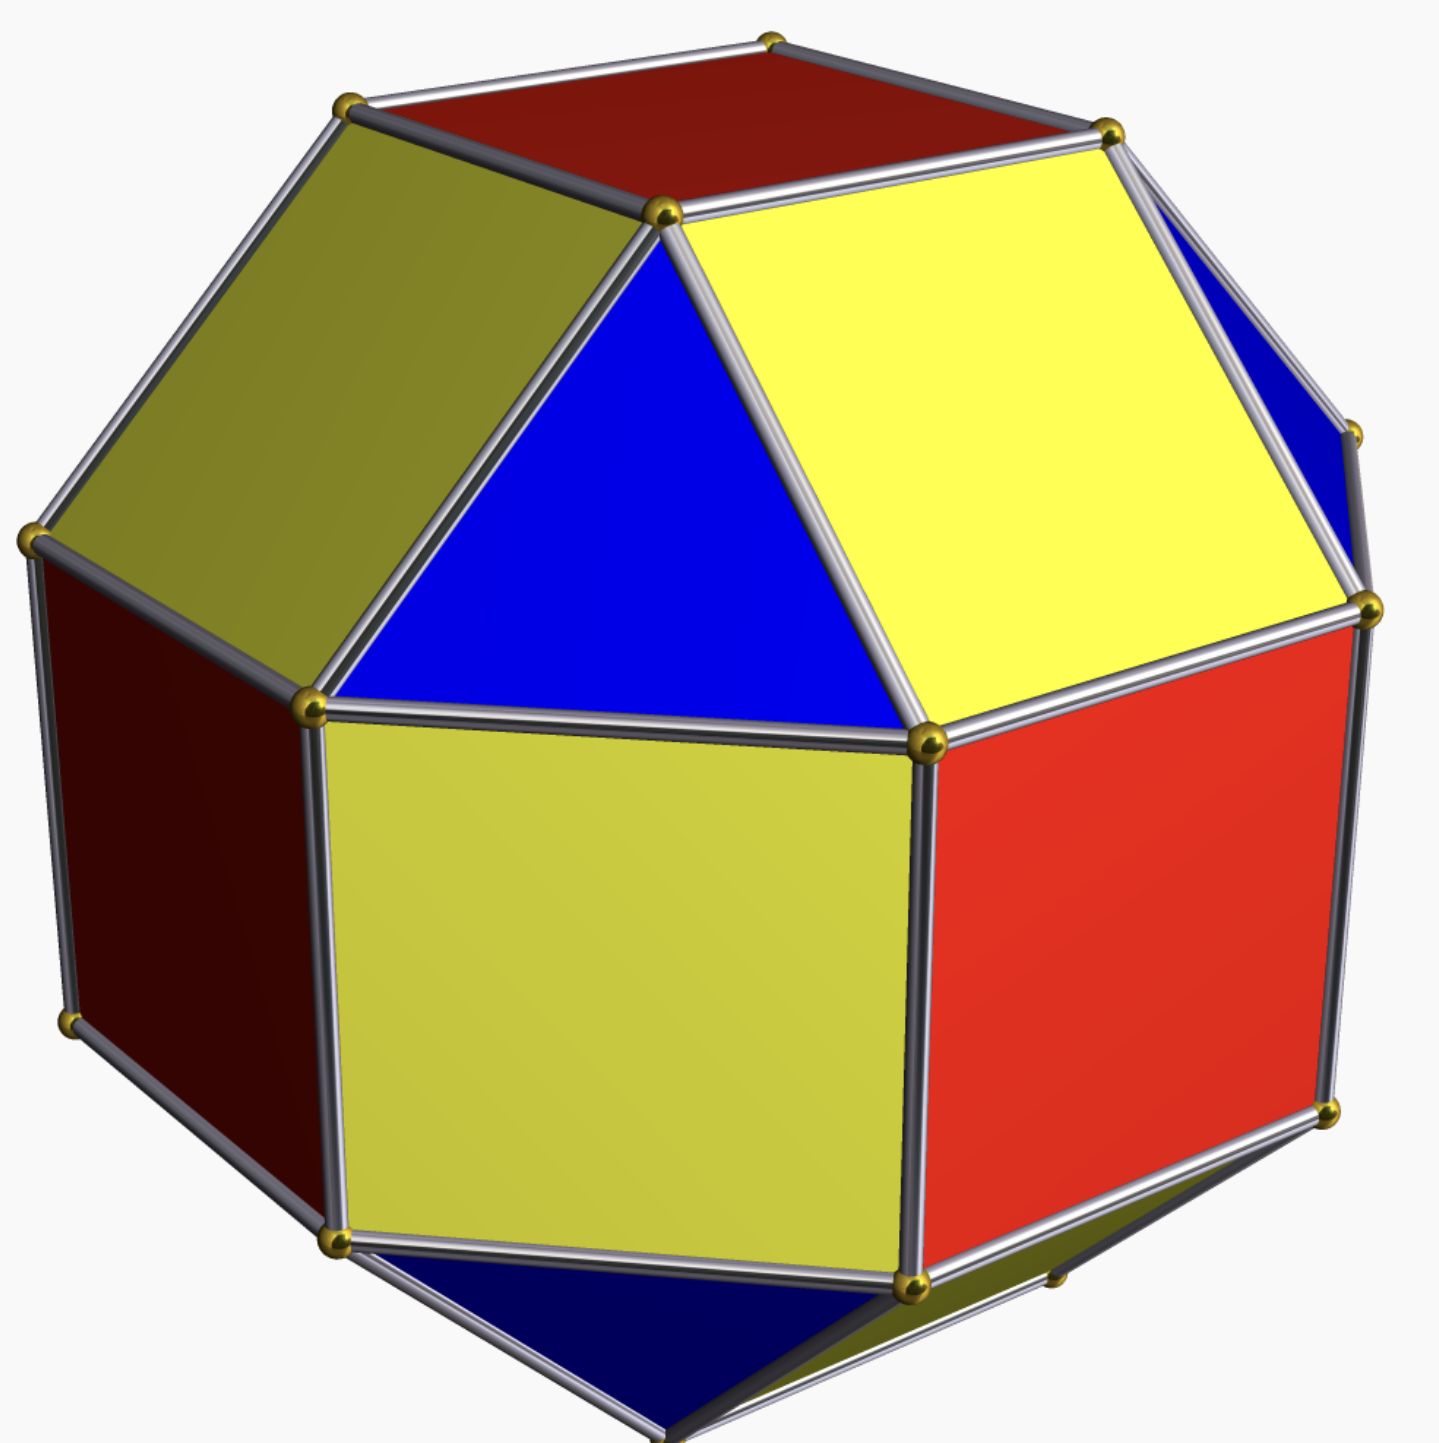
\includegraphics[width=\linewidth]{images/polyeder/Rhombenkuboktaeder.png}
        \caption{Rhombenkuboktaeder.}
        \label{fig:Rhombenkuboktaeder}
    \end{subfigure}
    \hfill
    \begin{subfigure}[b]{0.32\textwidth}
        \centering
        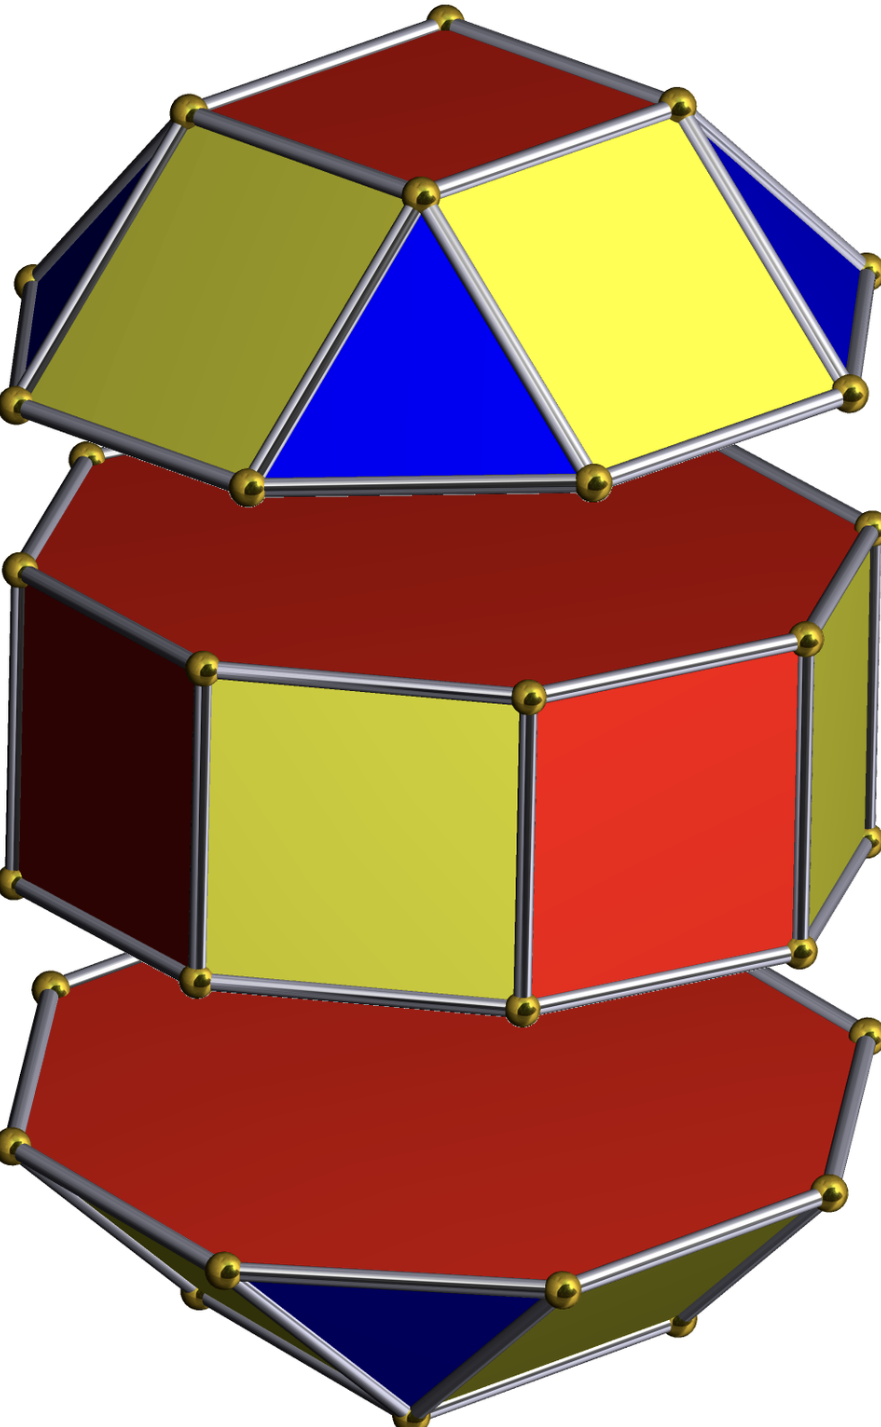
\includegraphics[width=\linewidth]{images/polyeder/RhombenkuboktaederToPseudorhombicuboctahedron.png}
        \caption{Rhombenkuboktaeder zerlegt in ein Prisma und zwei Dome.}
        \label{fig:RhombenkuboktaederZerlegt}
    \end{subfigure}
    \hfill
    \begin{subfigure}[b]{0.32\textwidth}
        \centering
        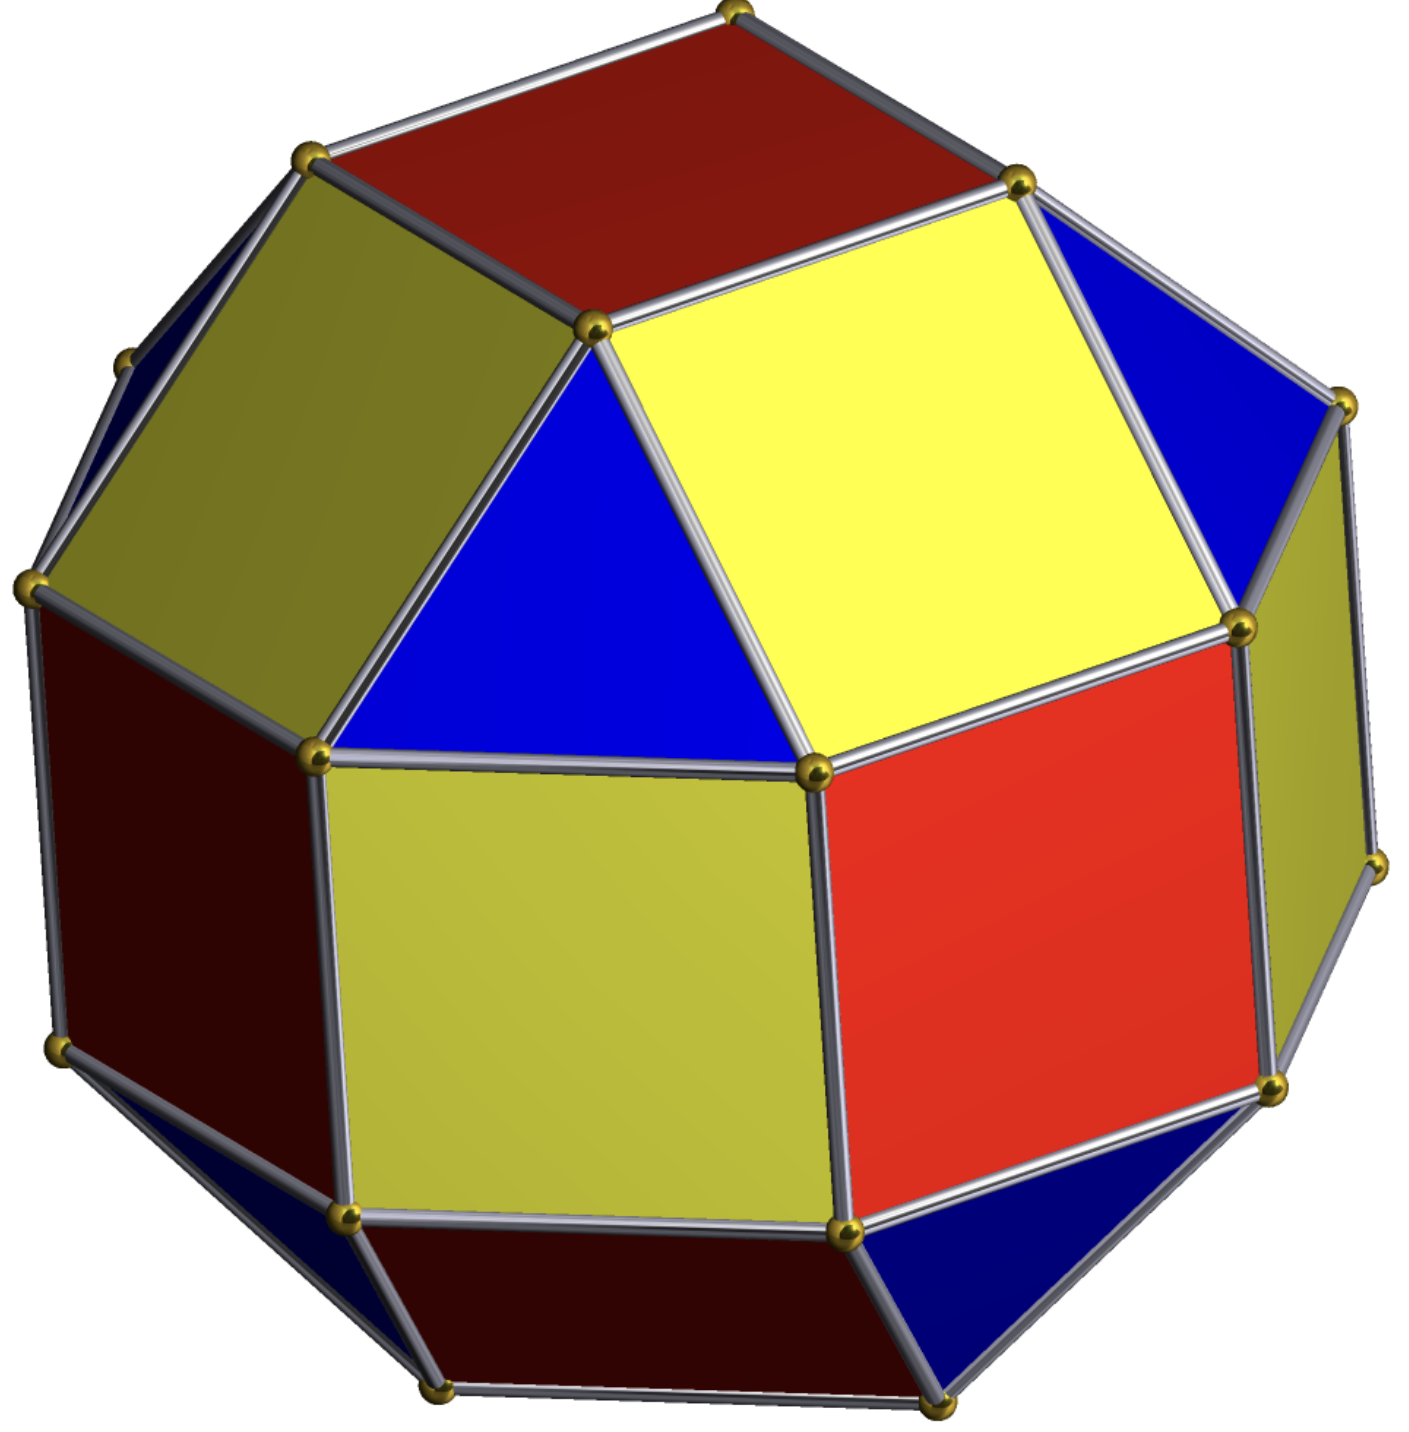
\includegraphics[width=\linewidth]{images/polyeder/Pseudorhombicuboctahedron.png}
        \caption{Pseudo-Rhombenkuboktaeder.}
    \end{subfigure}
    \caption{Rhombenkuboktaeder zu Pseudo-Rhombenkuboktaeder, Wikipedia \cite{elongated_square_gyrobicupola}.}
    \label{fig:rhombenkuboktaederToPseudorhombicuboctahedron}
\end{figure}